\section{Conclusion}

\subsection{Answer of Research Question}

\paragraph{Can Semantic Text Similarity including string-based and vector space models methods be used to find related articles? How effective and efficient is the metrics of performance, such as precision and operational time?}
\paragraph{How does the methods work in the practical scenario that the corpus keeps increasing with time? How is the performance of the incremental system different from a constant system? }
\paragraph{Is it useful to combine the STS methods? Does it yield to an improvement in performance or to a significant decrease of runtime?}
\paragraph{The above introduced methods are unsupervised and ignore other meta-data. Does it lead to an improvement with utilizing supervised or semi-supervised algorithms which are proposed in the field of learning to rank?}
通过逐一回答research question的方式总结整篇文章

\subsection{Application in Reality}
如果将系统实际使用,考虑到现在可以达到的准确率,无法实现完全自动化,可选取五个作为备选,然后人工选择,这一操作也可以大大提高准确率和减少工作量。

\begin{figure}[!htb]
    \centering
    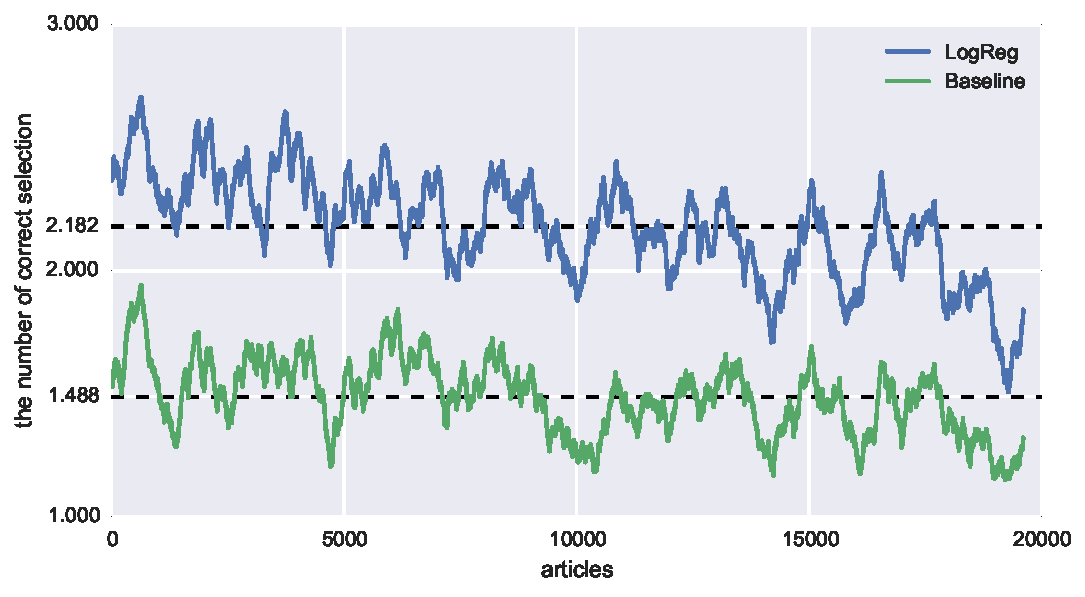
\includegraphics[width=\textwidth]{fig/precision_inc_supervised_5}
    \caption[]{}
    \label{fig:top5}
\end{figure}

\subsection{Future Work}
首先说明系统设计中的lack,即存在比较大的bias,因为我们主观的将discover related articles的过程简化为计算STS并combine with meta-data relevance. 这个做法会产生较大的bias, errors are reported in section 5. Future work 是可以使用其他的附加方法,来减少或者消除bias,在更精确的同时,达到覆盖更恰当的范围。
